\section{Implementation}
\label{sec:implementation}

\subsection{System Design}

Backscattered photocurrents from lasers are typically very low in intensity. How low depends on the situation. A low noise and high gain first stage amplifier is necessary to achieve the required output signal.  We gain intuition of the current required by measuring the induced photocurrent from the backscattered light of a laser pointer. 

\subsection{Camera Sensor Proof of Concept}
A Thorlabs Amplified Photodiode is used as the detector and a Keithley High Precision Multimeter measures its output as in \ref{fig:cam2}.

\begin{figure}[t]
  \centering
  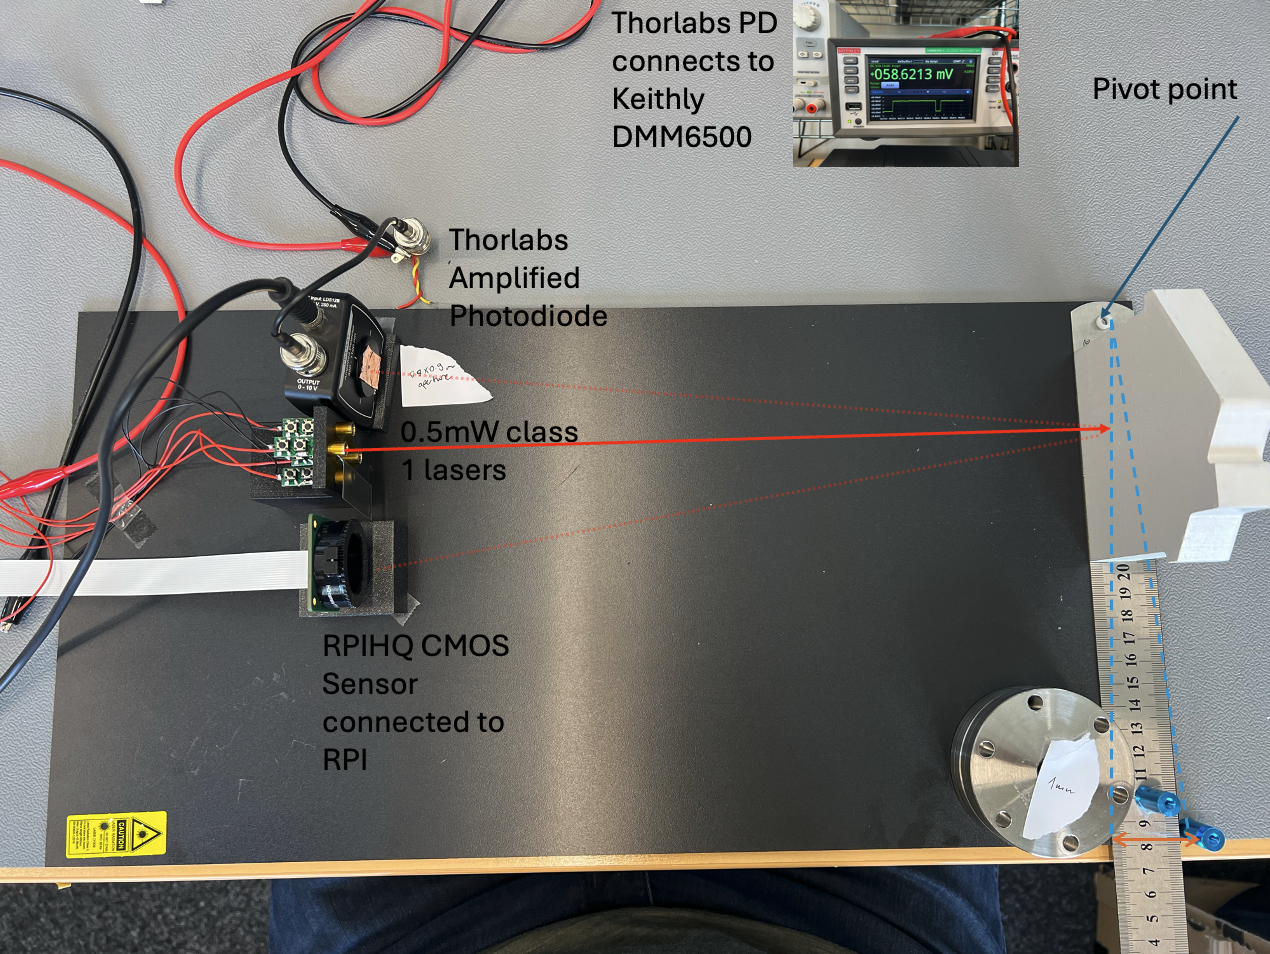
\includegraphics[width=\widthnarrow]{figures/impl/camera_setup.png}
  \caption{A laser is pointed at a painted wooden surface. A multimeter measured the current from a masked photodiode. A RPI HQ camera is used as a reference to visualise the speckle pattern).}
  \label{fig:cam1}
\end{figure} 


\begin{figure}[t]
  \centering
  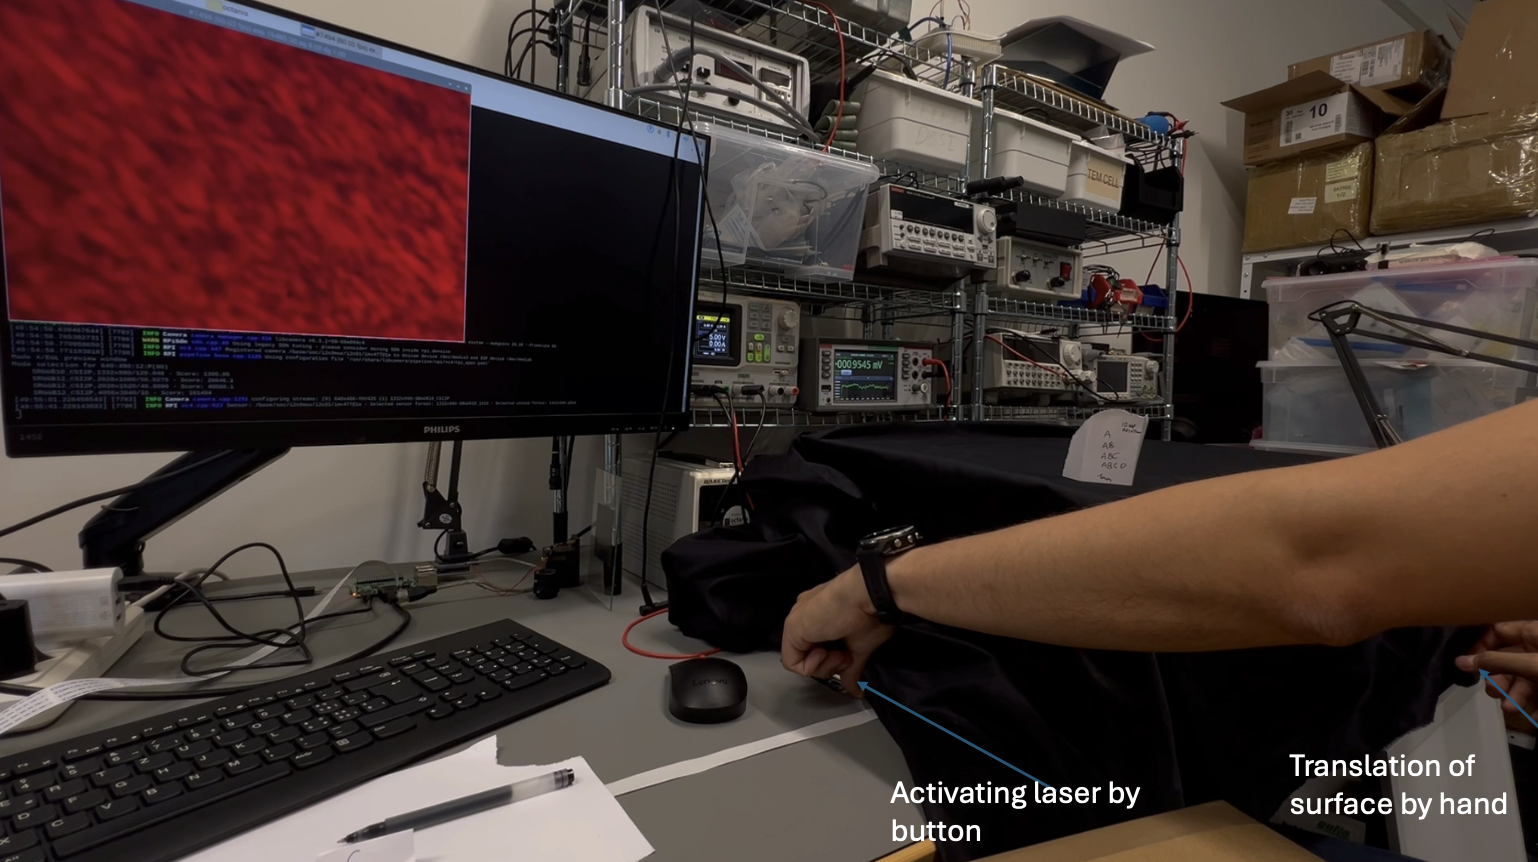
\includegraphics[width=\widthnarrow]{figures/impl/camera_setup2.png}
  \caption{Speckle pattern visualised by RPI Cam HQ (from Setup in \ref{fig:cam1})}
  \label{fig:cam2}
\end{figure}

A typical store-bought class 1 red laser pointer has an output power under 0.5mW. Using this laser pointer we find that the amount of photocurrent produced by the masked (0.9mm x 0.9mm pinhole) photodiode is on the order of 1 nA. This means that we need to at least be able to measure currents on this order of magnitude.

The active area of the photodiode determines the capacitance but also the current sensitivity. The capacitance directly influences possible bandwidth. Ideally, we want a small photodiode area and we find this in the VEMD2704 with 1.5mm^2 active area.

We choose a 3x3 grid of photodiodes. We validate this choice by recording a video of the speckle pattern using a Raspberry Pi HQ camera. In the video, the speckle pattern translates back and forth. The sensor area of the RPI Cam is large enough to accomodate 9 VEMD2704 photodiodes as in \ref{emulated1}. Using this emulation we can process the 9 area's average pixel intensity and create a 1d signal (coarsensess) \ref{emulated2}.

\begin{figure}[t]
  \centering
  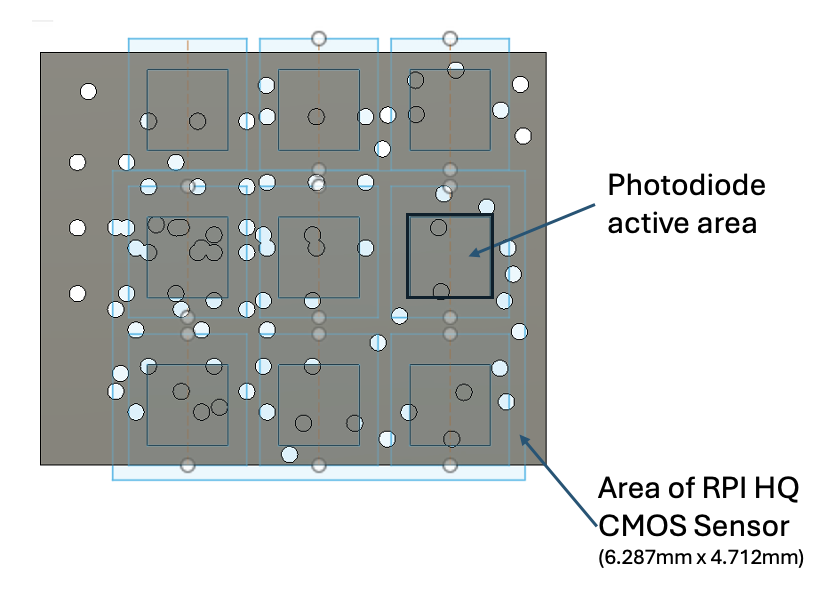
\includegraphics[width=\widthnarrow]{figures/impl/emulated1.png}
  \caption{Emulated array for validation.}
  \label{fig:emulated1}
\end{figure}

\begin{figure}[t]
  \centering
  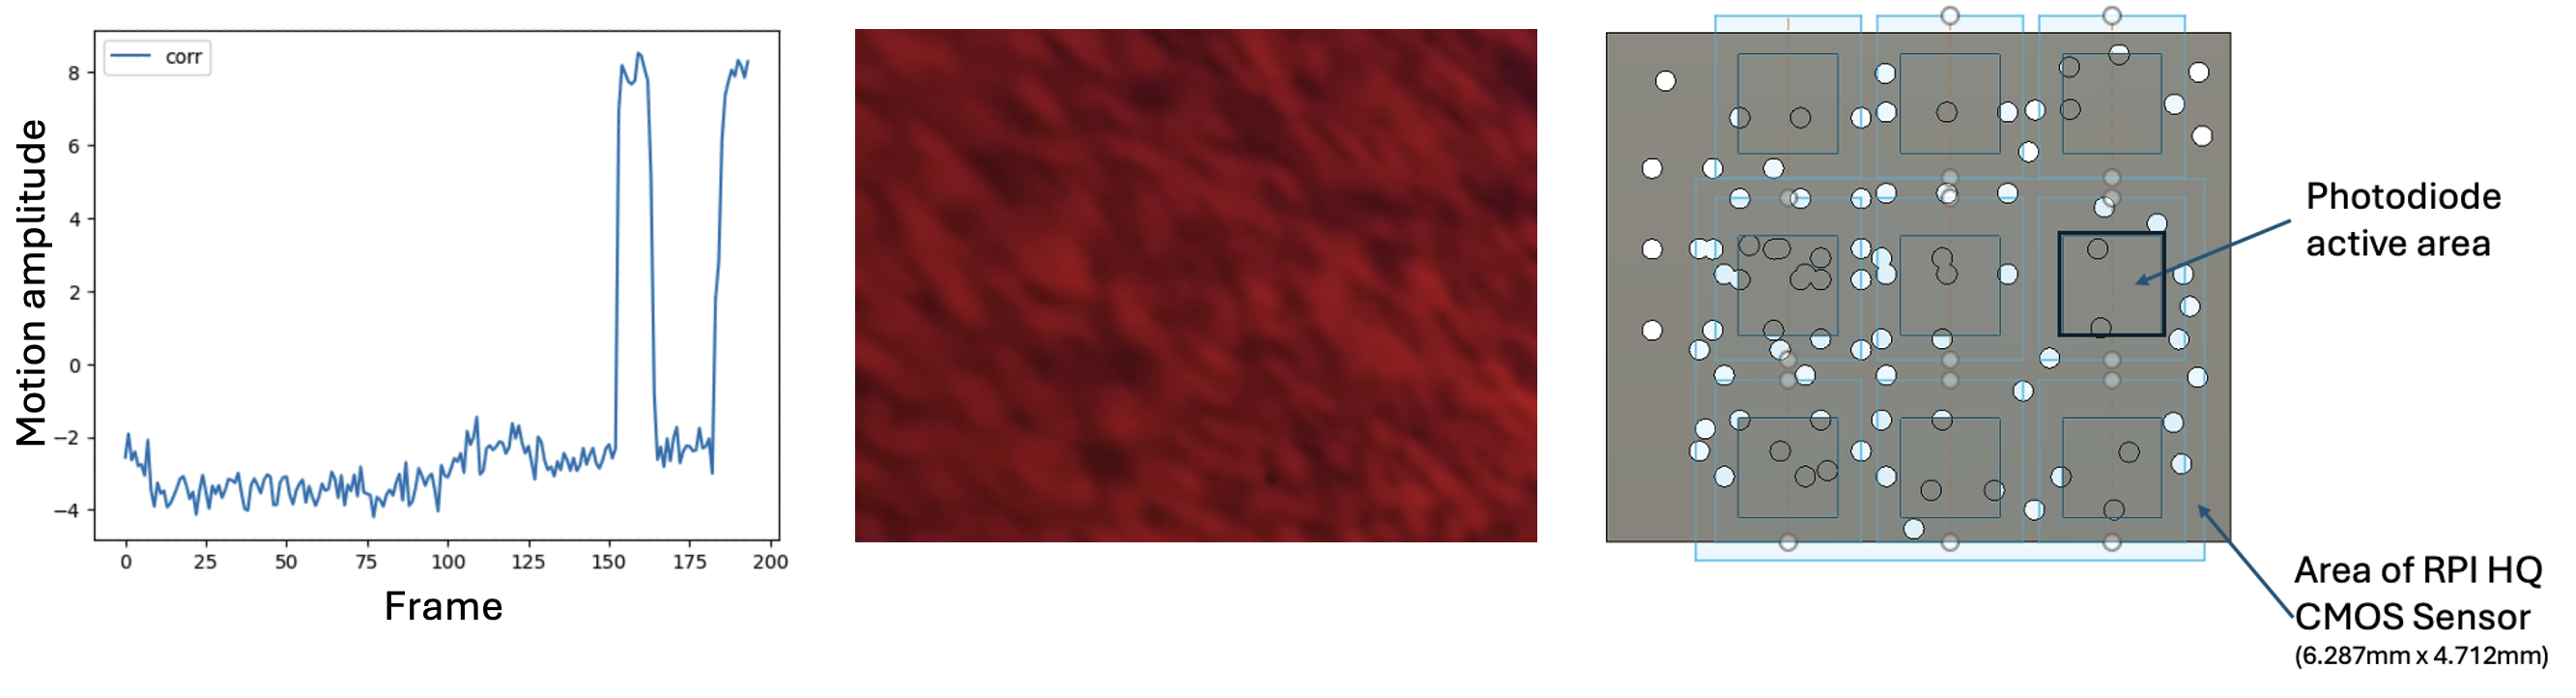
\includegraphics[width=\widthnarrow]{figures/impl/emulated2.png}
  \caption{Emulation captures translations of the speckle}
  \label{fig:emulated2}
\end{figure}

%- how many photodiodes can we use? how small can we get them to be? area of photodiodes ==> how much photocurrent. therefore, setup an experiment with a RPI HQ camera sensor and see view the resulting speckle pattern. 
%translate the house and watch the speckle pattern translate too. use red laser as the wavelength doesnt for easy experimentation.

%video of the speckle pattern motion

\subsection{Hardware Implementation}

The system block system block diagram is given in \ref{fig:block} using the order of magnitude values devised in the emulation.
\begin{figure}[t]
  \centering
  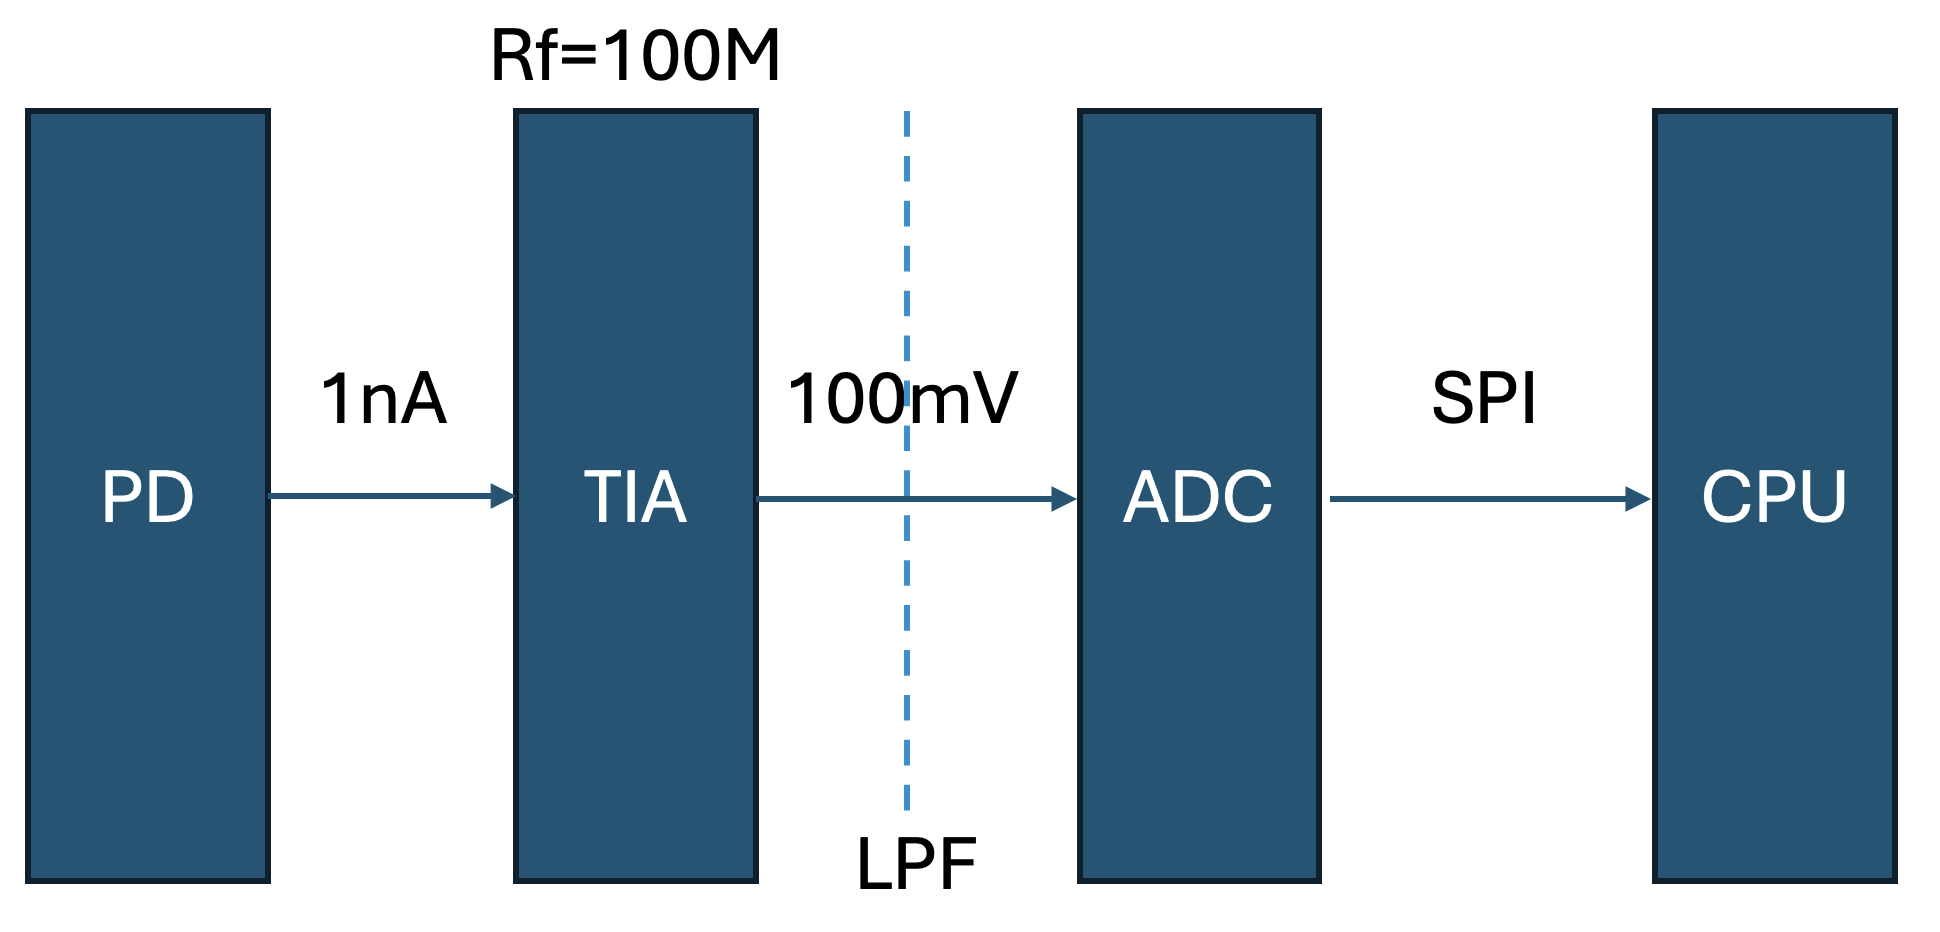
\includegraphics[width=\widthnarrow]{figures/impl/block_diagram.png}
  \caption{Block diagram}
  \label{fig:block}
\end{figure}

Photodiodes are commonly amplified using a transimpedance amplifier (TIA), although alternative options exist, such as current integrators like the DDC118. This application focuses on capturing high-frequency signals of up to 1 kHz, necessitating specific requirements for the operational amplifiers (op-amps) used.

The essential requirements for the op-amps include:
\begin{itemize}
  \item A minimum of two op-amps in a single package.
  \item A target price of approximately \$5 per chip.
  \item JFET input with low input capacitance.
  \item Capability to operate on a single power supply.
\end{itemize}

The OPA2380 fulfilled these requirements and a PCB was designed and built according to the datasheet recommendations. Particular attention to leakage currents was taken, like the implementation of a guard ring. The guard ring is a low impedance path for any stray AC that might want to make its way into the feedback path of the amp. The PCB is shown in \ref{fig:pcb} and contains a modular photodiode array with bandpass filter.

The bandpass filter is chosen to be at 850nm as that is where silicon photodiodes are most efficient. Lasers are 850nm are common and we are able to filter out a lot of environmental light.


\subsection{Signal Processing}

In this project, a Raspberry Pi 5 (RPI) was used with two types of Analog-to-Digital Converters (ADC).

The first ADC was unable to sample at high enough frequencies. Although it utilized a multiplexer (MUX), the channel switching was controlled via SPI, making it challenging to manage the switching delay. This limitation introduced a significant amount of noise, which was also noted in several GitHub issues reported by users.

A second ADC was then tested, featuring a higher sample rate and advertised synchronous sample readout capability. This ADC is designed as a Raspberry Pi HAT and uses the Pi's 5V supply as its analog reference. However, this reference is very noisy, with peak-to-peak noise in the millivolt range. To mitigate this issue, a bench power supply was used to power the ADC externally.

Raw data from the ADC was recorded and observed in real-time or processed post-capture. Real-time observations were conducted while simultaneously monitoring the speckle camera and the infrared (IR) camera.



%wide figs

\begin{figure*}[t]
  \centering
  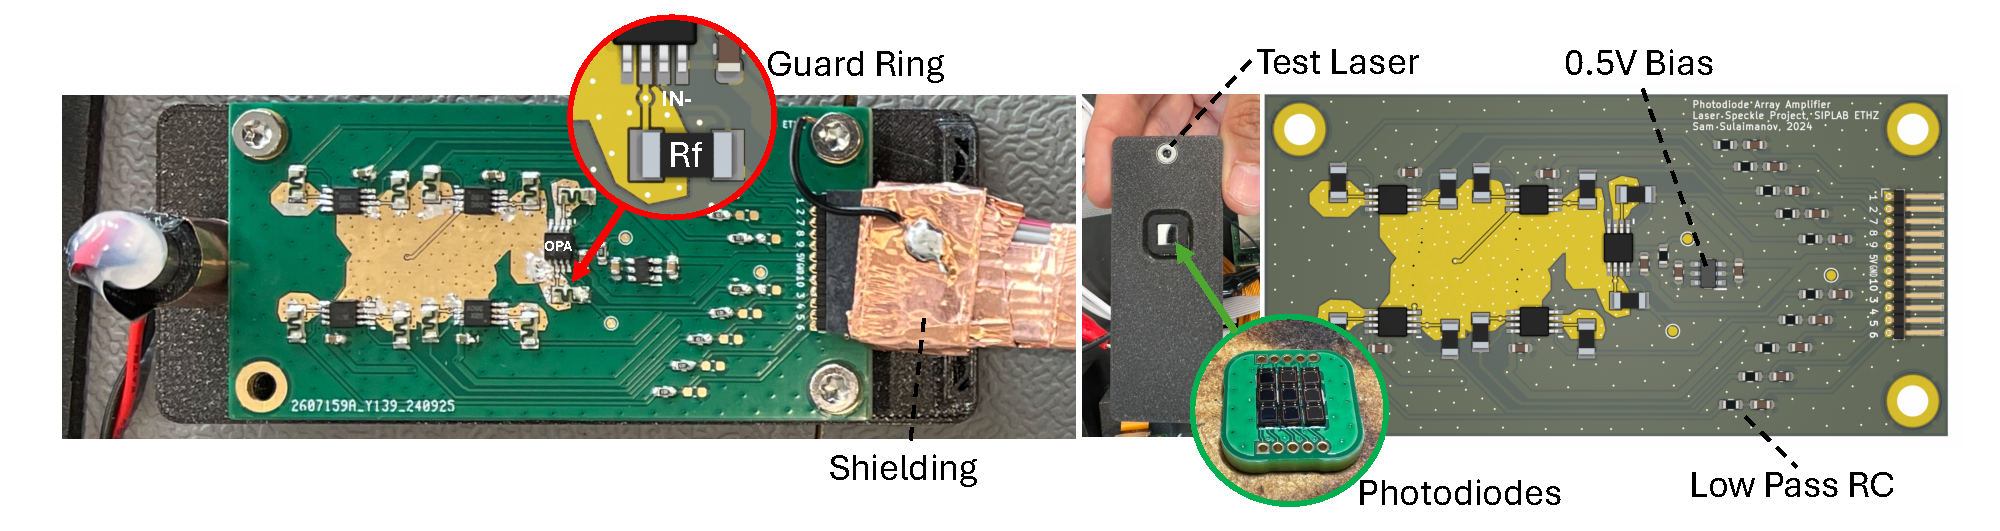
\includegraphics[width=\textwidth]{figures/impl/pcb_design.pdf}
  \caption{maxwidth cap}
  \label{fig:pcb}
\end{figure*}
